
\section{Nền tảng iOS và các thành phần cơ bản}
iOS là hệ điều hành di động do Apple phát triển, được sử dụng chủ yếu trên các thiết bị như iPhone, iPad và iPod Touch. Với kiến trúc nhiều tầng cùng hệ sinh thái phong phú, iOS cung cấp môi trường ổn định, bảo mật và hiệu năng cao cho việc phát triển ứng dụng di động. Để xây dựng một ứng dụng iOS hiệu quả, lập trình viên cần nắm vững các thành phần cơ bản như vòng đời ứng dụng, delegate, giao diện người dùng, cũng như các mô hình kiến trúc phổ biến. Phần này sẽ trình bày tổng quan về các yếu tố cốt lõi tạo nên nền tảng iOS và vai trò của chúng trong quy trình phát triển ứng dụng.
    \subsection{Kiến trúc tầng của iOS}
        \begin{flushleft}
            \begin{figure}[H] % hoặc [h], [t], [b] tùy vị trí
                \centering
                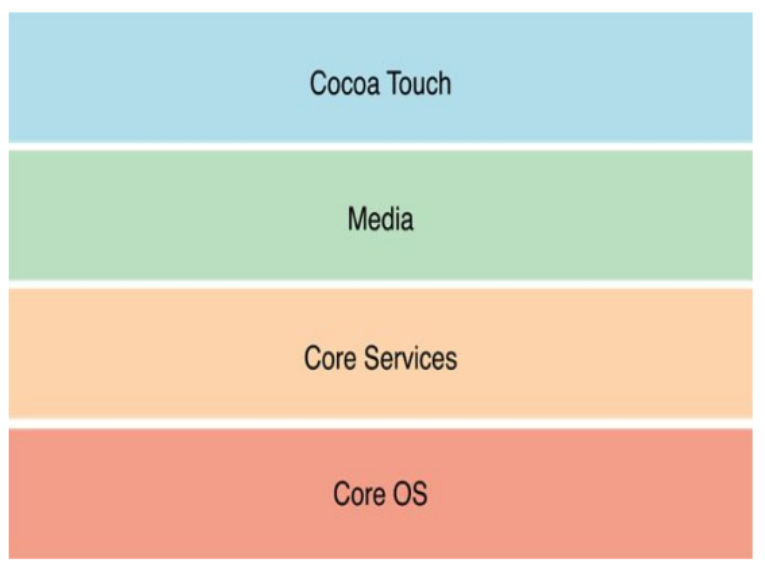
\includegraphics[width=0.8\textwidth]{images/kientrucios.png}
                \caption{Kiến trúc phân tầng IOS\cite{kientrucios}.}
                \label{fig:kientrucios}
            \end{figure}

            Hệ điều hành iOS được tổ chức theo kiến trúc nhiều tầng, trong đó mỗi tầng đảm nhận một vai trò cụ thể và cung cấp các framework cũng như dịch vụ khác nhau. Ở tầng cao nhất, \textbf{Cocoa Touch} cung cấp các framework cốt lõi dành cho việc xây dựng giao diện người dùng, đáng chú ý là \textit{UIKit} và \textit{SwiftUI}. Các công nghệ đồ họa, âm thanh và video như \textit{Core Graphics}, \textit{Core Animation}, và \textit{AVFoundation} được tập trung tại tầng \textbf{Media}, giúp xử lý các chức năng đa phương tiện. Bên dưới đó, tầng \textbf{Core Services} cung cấp các dịch vụ nền tảng cần thiết như \textit{Core Data} để quản lý dữ liệu, \textit{Core Location} để định vị, và \textit{Foundation framework} cho các chức năng cơ bản. Cuối cùng, tầng \textbf{Core OS} đóng vai trò là nền tảng thấp nhất của hệ điều hành, nơi tích hợp kernel, hệ thống tệp, các cơ chế bảo mật và các dịch vụ hệ thống cấp thấp.

       
        \end{flushleft}
   \subsection{ Vòng đời ứng dụng IOS}	
        \begin{flushleft}
            Khi người dùng khởi động điện thoại, chỉ có các thành phần của hệ điều hành (\textit{Operating System}) được phép hoạt động, trong khi các ứng dụng của người dùng chưa được kích hoạt. Các ứng dụng, bao gồm cả ứng dụng của bạn, sẽ chỉ bắt đầu thực thi khi người dùng nhấn vào biểu tượng ứng dụng trên màn hình chính. Chính lúc đó, \textbf{Springboard} – trình quản lý giao diện màn hình chính của iOS – sẽ chịu trách nhiệm kích hoạt ứng dụng. Ứng dụng cùng với các thư viện liên quan sẽ được tải vào bộ nhớ và bắt đầu khởi chạy, trong khi đó \textbf{Springboard} sẽ hiển thị màn hình khởi động (launch screen) để tạo cảm giác phản hồi tức thì cho người dùng. Sau khi quá trình tải hoàn tất, ứng dụng sẽ bắt đầu thực thi, và \texttt{AppDelegate} – đối tượng chịu trách nhiệm quản lý vòng đời của ứng dụng 
            – sẽ nhận được các thông báo tương ứng từ hệ thống.
            Trong quá trình hoạt động, ứng dụng iOS luôn ở một trong các trạng thái xác định: \textbf{Not Running}, \textbf{Inactive}, \textbf{Active}, \textbf{Background}, hoặc \textbf{Suspended}. Những trạng thái này phản ánh tình huống hiện tại của ứng dụng đối với hệ điều hành, và tại bất kỳ thời điểm nào, ứng dụng của bạn đều sẽ nằm trong một trong các trạng thái đó. Việc hiểu rõ và xử lý đúng các trạng thái này là yếu tố then chốt để đảm bảo ứng dụng vận hành hiệu quả, tiết kiệm tài nguyên và mang lại trải nghiệm người dùng mượt mà.
            
        \end{flushleft}
        \begin{figure}[H] % hoặc [h], [t], [b] tùy vị trí
            \centering
            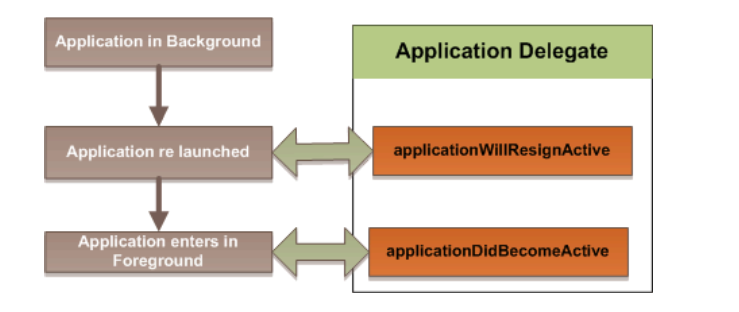
\includegraphics[width=0.8\textwidth]{images/vongdoiios.png}
             \caption{Vòng đời ứng dụng IOS\cite{life cycle-IOS}.} 
            \label{fig:vongdoiios}
        \end{figure}
         \begin{flushleft}
            \textbf{NotRunning:}Ứng dụng chưa được khởi chạy hoặc đã bị hệ thống chấm dứt.
            \textbf{Inactive:} Ứng dụng đang chạy ở foreground nhưng không nhận events (ví dụ: khi có cuộc gọi đến).\\
            \textbf{Active:} Trạng thái bình thường khi ứng dụng chạy ở foreground và đang xử lý events.\\
            \textbf{Background:} Ứng dụng không hiển thị nhưng vẫn chạy và thực thi mã.\\
            \textbf{Suspended:} Ứng dụng ở background nhưng không chạy mã, có thể bị hệ thống chấm dứt để giải phóng tài nguyên.
         \end{flushleft}
         \subsection{App Delegate và Scene Delegate}
         Trong iOS, hai thành phần quan trọng đảm nhận việc quản lý vòng đời và giao diện của ứng dụng là \textbf{AppDelegate} và \textbf{SceneDelegate}. \textbf{AppDelegate}\cite{ App-Scene Delegate} chịu trách nhiệm xử lý các sự kiện cấp cao liên quan đến vòng đời tổng thể của ứng dụng, chẳng hạn như khi ứng dụng được khởi động, chuyển sang chế độ nền, hoặc bị chấm dứt. Bên cạnh đó, nó cũng đảm nhiệm các tác vụ cấu hình ban đầu như đăng ký notification, khởi tạo dịch vụ, và thiết lập dữ liệu dùng chung.
         Kể từ iOS 13, Apple giới thiệu khái niệm \textbf{Scene} để hỗ trợ việc chạy nhiều cửa sổ giao diện (\textit{multi-window}) trong cùng một ứng dụng, đặc biệt trên iPad. Chính vì thế, \textbf{SceneDelegate} ra đời nhằm tách riêng trách nhiệm quản lý giao diện người dùng (UI lifecycle) cho từng scene. \textbf{SceneDelegate} xử lý các sự kiện như scene được kết nối, hiển thị, vào nền hoặc bị hủy, từ đó cho phép quản lý độc lập từng cửa sổ ứng dụng.
         Sự phân tách giữa \texttt{AppDelegate} và \texttt{SceneDelegate} giúp ứng dụng có kiến trúc rõ ràng hơn, dễ dàng mở rộng cho các thiết bị hỗ trợ đa cửa sổ, đồng thời tuân thủ tốt hơn nguyên lý phân chia trách nhiệm trong lập trình.

         \subsection{Luồng làm việc của người dùng và Storyboards}

         Trong quá trình phát triển ứng dụng iOS, việc thiết kế luồng di chuyển của người dùng giữa các màn hình là một phần quan trọng nhằm đảm bảo trải nghiệm sử dụng mượt mà và trực quan. Để hỗ trợ việc này, Apple cung cấp công cụ trực quan gọi là \textbf{Storyboards}, cho phép lập trình viên dễ dàng thiết kế giao diện và quản lý mối quan hệ giữa các màn hình trong ứng dụng. Thông qua giao diện kéo thả, Storyboards giúp định hình toàn bộ hành trình người dùng chỉ trong một file duy nhất.
         Bên trong Storyboards, các chuyển tiếp giữa các màn hình được định nghĩa bằng \textbf{Segues}. Mỗi segue mô tả cách thức mà ứng dụng chuyển từ một view controller này sang view controller khác, chẳng hạn như chuyển tiếp theo kiểu push, modal hoặc custom. Các segue này có thể được thiết lập trực tiếp trong giao diện hoặc được kích hoạt thông qua mã lệnh.
         Bên cạnh phương pháp sử dụng Storyboards, một lựa chọn khác thường được sử dụng trong các dự án có yêu cầu tùy biến cao là \textbf{Programmatic UI}. Với phương pháp này, giao diện người dùng được tạo hoàn toàn bằng mã Swift mà không phụ thuộc vào file storyboard. Cách tiếp cận này mang lại sự linh hoạt tối đa, đặc biệt hữu ích trong các ứng dụng lớn, có tính tái sử dụng cao hoặc cần kiểm soát giao diện một cách chính xác hơn.
         Việc lựa chọn giữa Storyboards và Programmatic UI phụ thuộc vào mục tiêu của dự án, quy mô nhóm phát triển và yêu cầu kỹ thuật. Trong thực tế, nhiều dự án kết hợp cả hai cách tiếp cận để tận dụng ưu điểm của từng phương pháp.